\documentclass[../catalog.tex]{subfiles}

\begin{document}

\subsubsection{Problem}

As has been widely documented within the database community
(\cite{leis2015good}, \cite{lohman2014query}), many complex queries
are highly sensitive to join ordering. We have discussed the
established heuristical approaches originating from
\cite{selinger1979access} in \autoref{known-techniques} and hinted at
their various shortcomings.

There we concluded that in practice, cardinality estimation under the
traditional assumptions (uniformity, uncorrelated join predicates,
overlapping key domains, and full access to meaningful statistics) can
not avoid disastrous plans.

While improvements in probabilistic modeling of correlations, on-line
gathering of index statistics, and adaptive approaches to query
execution such as Eddies provide many interesting avenues of inquiry,
we are primarily interested in approaches that make disastrous plans
impossible — possibly at the expense of best- and average-case
performance.

The reasons for this are two-fold: first, and most importantly,
disastrous query plans violate all three of the desired properties
outlined in \ref{problem}. Second, from experiences with 3DF itself,
and other declarative systems such as the Prolog language, we know
that the mere \emph{possibility} of unpredictable, severe performance
degradations break the fundamental promise of the declarative
abstraction, and force users to reason defensively about the system
runtime.

We can further distinguish between different classes of problematic
queries:

\begin{itemize}

  \item \textbf{Worst-Case} Queries for which any join-at-a-time plan
    will process asymptotically more tuples than could possibly be
    contained in the result set. A class of queries for which this is
    case is formalized in \cite{ngo2012worst}. Intuitively, these are
    queries that compute the $d$-way join of all $(d-1)$-ary
    projections of the result set. An instance of this query class is
    the triangle query, which computes $(a,b,c)$ from its projections
    $(a,b)$, $(b,c)$, and $(a,c)$.

    Triangles and cyclic sub-pattern queries in general have many
    applications. The LDBC Social Network Benchmark query
    \texttt{BI/read/11}, for example, contains a triangle between
    comments, messages, and tags, in order to find unrelated
    replies. Query \texttt{BI/read/19} asks for a 4-clique between
    persons, comments, and messages, in order to determine for each
    person the set of strangers they have interacted with.

  \item \textbf{Average-Case} Queries across correlated columns,
    i.e. on data where the assumptions of uniformity, independence,
    and overlapping domains are violated to varying extents. For
    queries in this class, accurate estimation of cardinalties can
    make a huge difference for join-at-a-time plans. These are queries
    whose hypergraph representation is cycle-free.

    LDBC query \texttt{BI/read/2}, for example, joins countries,
    cities, persons, messages, and tags. The order of this traversal
    can make a significant difference, depending on the relative
    selectivity, and additional predicates applied to individual
    relations (e.g. ``consider only cities in germany'').

  \item \textbf{Best-Case} Queries across uncorrelated, uniformly
    distributed columns. Their hypergraph representation is
    cycle-free, and the assumptions of traditional cardinality
    estimatino hold. These are best-case queries and as such, rare in
    practice.

    Examples would be star-joins on uncorrelated columns, where each
    column holds at most a fixed number of values for each
    key. E.g. joining user ids exclusively on single-cardinality
    attributes such as username, email, or age.
    
\end{itemize}

\subsubsection{Remedy}

We covered recent advances in the area of worst-case optimal join
processing that introduce n-way join algorithms with improved
asymptotic complexity for queries in the worst-case class. These
algorithms distinguish themselves from traditional approaches, by
estimating cardinalities for individual tuples. For average- and
best-case queries we thus expect a worst-case optimal approach to
match or outperform a heuristics-based approach in terms of the number
of tuples processed, but potentially with significant constant
overheads.

Our implementation of a worst-case optimal dataflow join operator is
detailed in \autoref{impl-hector}.

\subsubsection{Evaluation}

First, we want to examine whether a worst-case optimal join strategy
does lead to more predictable latencies, \emph{irrespective of the
  clause order provided by the user}. For this we will consider the
triangle query \texttt{[?a :edge ?b] [?b :edge ?c] [?a :edge ?c]} on
the livejournal graph. The graph contains 68 million edges. We
introduce edges in node order, feeding them into a single
attribute. The i-th round of input is therefore that in which all
edges starting at node i are ingested. We use a single worker, running
on a single core of a 2.7 GHz Intel Core i5, with 16GB RAM available.

We run this setup for both strategies — consecutive binary joins
(\emph{JoinJoinJoin}) and worst-case optimal (\emph{Hector} — and for
three different input clause orders each, measuring completion time
for each round of inputs. The resulting latency distributions are
shown in figure \ref{fig:triangle-cdfs}.

\begin{figure}[h!]
  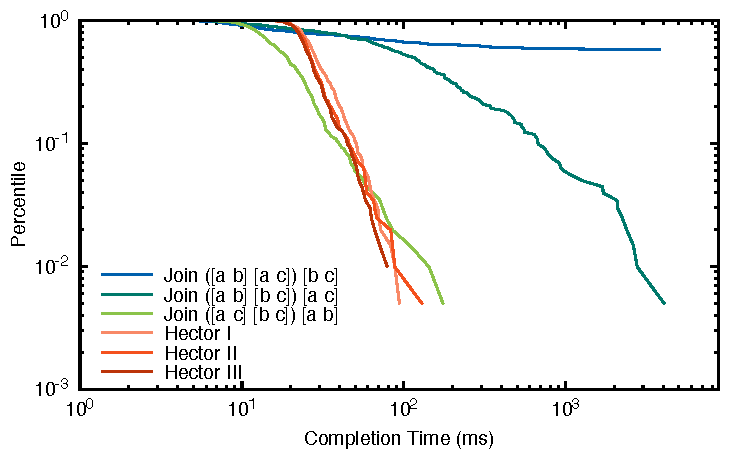
\includegraphics[width=1.0\linewidth]{results/triangles/out/all_cdfs}
  \caption{Triangle Query - Latency CCDFs}
  \label{fig:triangle-cdfs}
\end{figure}

As expected, we observe that performance of the JoinJoinJoin strategy
is highly sensitive to clause order. In particular, the first ordering
(\texttt{([a b] [a c]) [b c]}), runs out of memory at node 87, while
the third ordering (\texttt{([a c] [b c]) [a b]}) consistently
outperforms all of the tested strategies.

The worst-case optimal strategy performs consistently well for all
three input clause orderings and consistently outperforms the two
disastrous join orderings by one to many orders of magnitude. The best
performing JoinJoinJoin order can outperform Hector, but with a
similar long-tail and twice the maximum latency. [@TODO percentile
  table]

Figure \ref{fig:triangle-cdfs-extended} shows that these observations
remain valid when measuring thrice the number of rounds, as well as
when increasing the batch size to introduce one thousand nodes at a
time.

\begin{figure}[h!]
  \begin{subfigure}{.5\textwidth}
    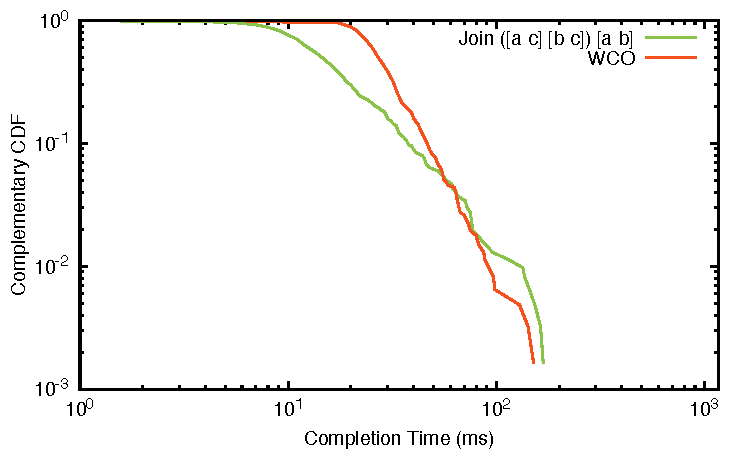
\includegraphics[width=1.0\linewidth]{results/triangles/out/extended_cdf}
    \caption{More Rounds}
  \end{subfigure}
  \begin{subfigure}{.5\textwidth}
    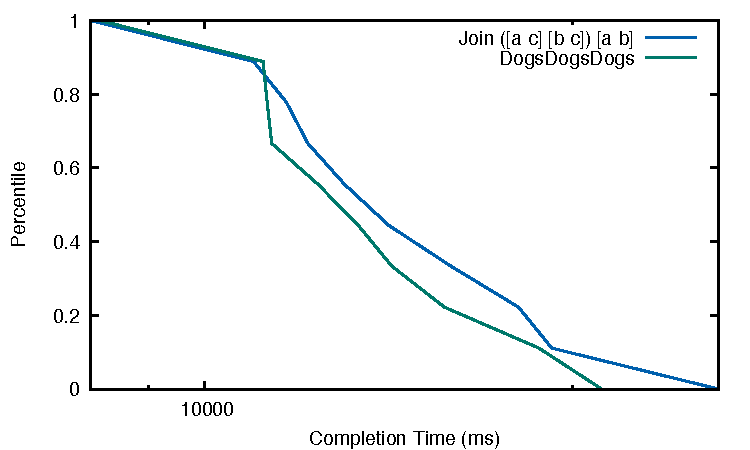
\includegraphics[width=1.0\linewidth]{results/triangles/out/batch_cdf}
    \caption{Batch Size 1000}
  \end{subfigure}

  \label{fig:triangle-cdfs-extended}
\end{figure}

\end{document}
